%!TEX root = ../main.tex
%-------------------------------------------------------------------------------
% 								BAB I
% 							LATAR BELAKANG
%-------------------------------------------------------------------------------

\chapter{PENDAHULUAN}

\section{Latar Belakang Masalah}

% Paragraph 1
Perkembangan teknologi pada bidang informasi pada era ini sangatlah pesat. 
Hampir semua kalangan masyarakat dapat menggali informasi di mana pun dan kapanpun 
selagi terhubung dengan koneksi internet. Salah satu perkembangan teknologi di bidang 
informasi yang paling berperan adalah \emph{search engine}. Dengan \emph{search engine}, 
pengguna dapat mencari informasi yang diinginkan dengan cara mengetikkan 
\emph{keyword} dari informasi yang dicari. \emph{Search engine} akan menampilkan semua 
informasi yang relevan berdasarkan \emph{website} yang mengandung \emph{keyword} dari yang 
pengguna cari. Setelah menampilkan \emph{website} yang relevan, pengguna dapat melihat 
lebih detail terkait informasi yang dicari dengan mengunjungi \emph{website} tersebut. 
Selain memiliki manfaat bagi pengguna, \emph{search engine} juga bermanfaat bagi 
pemilik \emph{website} karena dapat menambahkan jumlah pengunjung \emph{website} setiap 
saat tanpa perlu melakukan promosi ataupun iklan.

% Paragraph 2
Terdapat penelitian yang berkaitan dengan \emph{search engine} yang belum lama telah dibuat, 
di antaranya adalah penelitian mengenai \emph{crawler} berjalan secara \emph{multi-threaded} (\cite{fathan2021crawler}). 
Penelitian ini dilanjutkan dengan melakukan \emph{refactoring}  pada \emph{crawler} dan menambahkan 
pencarian \emph{similiarity score} dari halaman \emph{web} hasil \emph{crawling} (\cite{lazuardy2023}).  Lalu 
penelitian ini dilanjutkan dengan mengembangkan \emph{crawling engine} yang berjalan secara 
terdistribusi yang akan mengimplementasikan penggunaan \emph{socket} dalam mendistribusikan tugas 
ke setiap \emph{slave machines} (\cite{ridho2024}). \emph{Crawling} terdistribusi diterapkan dengan melakukan 
pemecahan \emph{crawling} terhadap mesin yang berbeda. Hal ini berguna untuk meringankan beban 
kerja yang dijalankan pada masing-masing mesin. Selain meringankan beban kerja, mesin yang 
berjalan juga akan menghasilkan \emph{crawling} dalam jumlah masif yang lebih efisien. 

% Paragraph 3
Meninjau hasil akhir dari percobaan penelitian sebelumnya (\cite{ridho2024}),  terdapat kelemahan 
yang harus diperbaiki pada penyimpanan data. Berikut adalah gambar arsitektur sistem 
terdistribusi yang dibuat oleh penelitian sebelumnya (\cite{ridho2024}).

\begin{figure}[H]
  \centering{}
	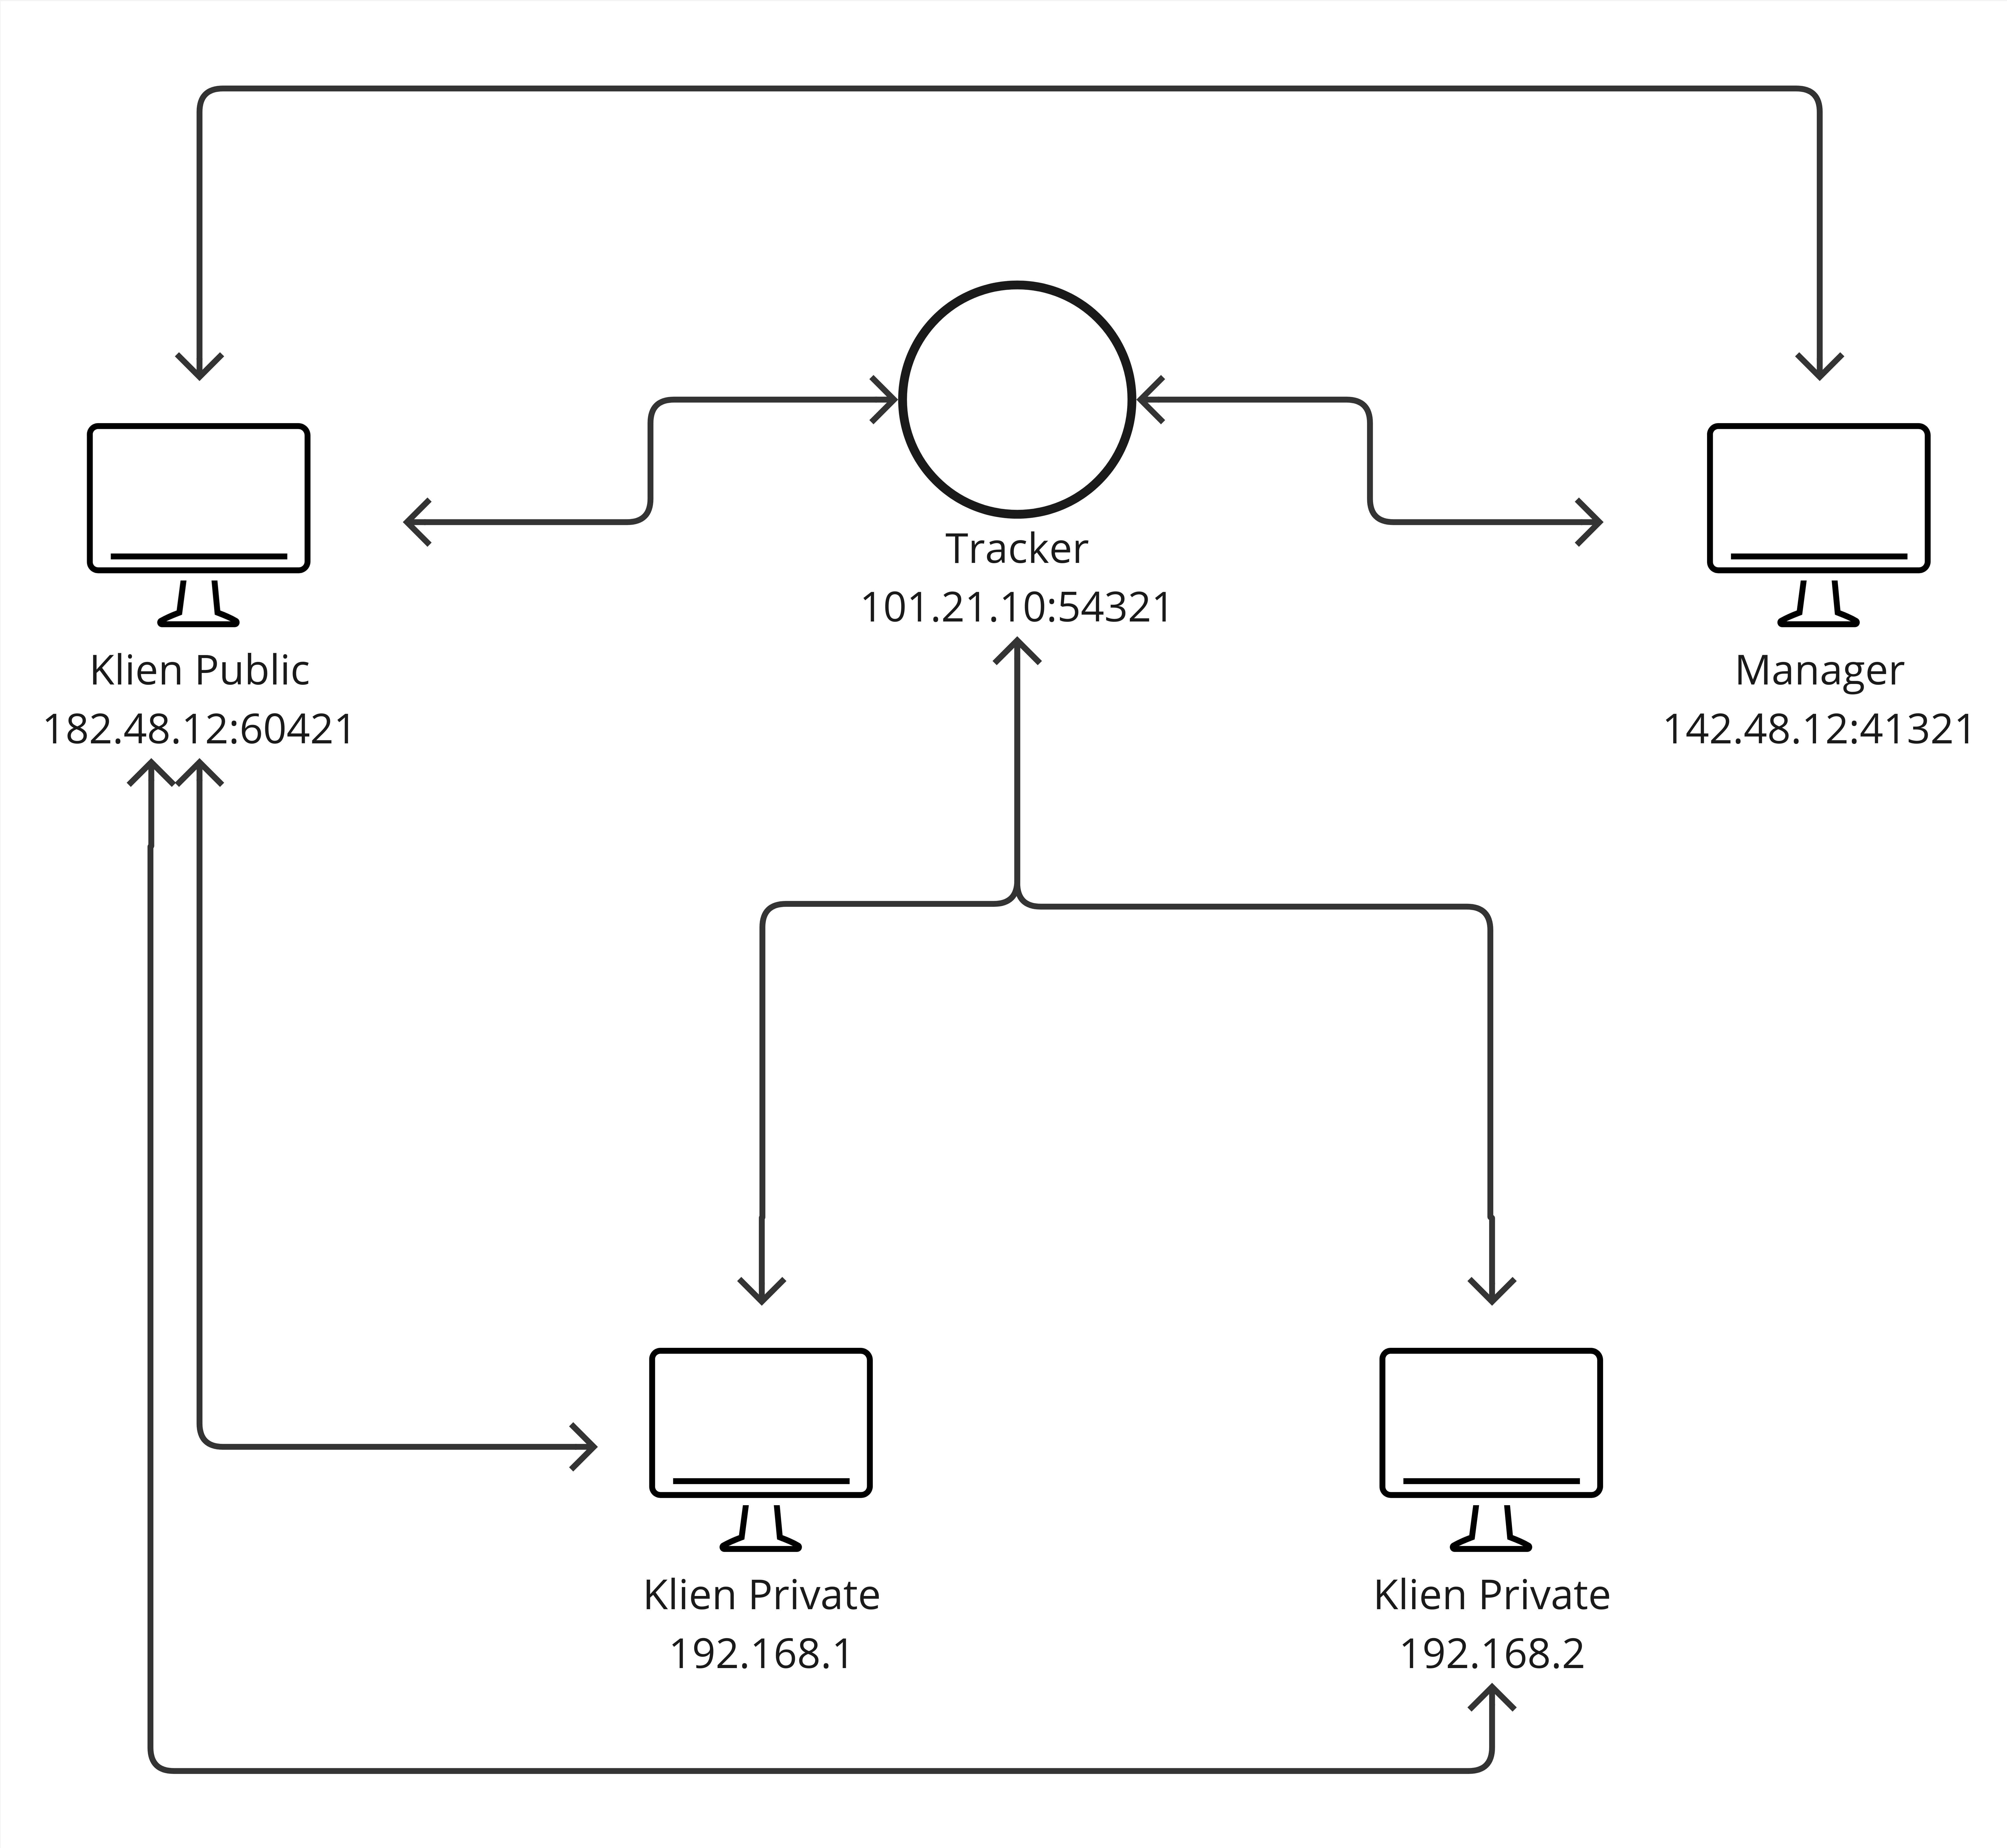
\includegraphics[width=0.85\textwidth]{gambar/bab1/arsitektur_baru}
  \caption{Arsitektur Sistem \emph{Crawler} Terdistribusi Sebelumnya (\cite{ridho2024})} 
\end{figure}

% Paragraph 4
Pada arsitektur tersebut \emph{database} disimpan secara terpusat pada 1 \emph{public 
client} walaupun masing-masing \emph{private client} juga menyimpan data. Akan 
lebih baik jika penyimpanan dilakukan secara terdistribusi daripada 
harus terpusat. Berdasarkan \emph{Paper An Overview of Distributed Databases} (\cite{overviewdistributed})
dinyatakan bahwa salah satu manfaat dari penerapan \emph{database} terdistribusi 
ini adalah \emph{High Performance-Queries and updates are largely local so that 
there is no network bottleneck}. Berdasarkan pernyataan tersebut didapatkan 
bahwa \emph{database} terdistribusi membuat performa \emph{query database} terutama \emph{query} 
yang jumlahnya cukup besar akan menjadi lebih efektif serta akan terhindar 
dari \emph{network bottleneck} karena operasi penyimpanan atau pengubahan dilakukan 
secara lokal. Terdapat manfaat lain yang dinyatakan di \emph{paper} tersebut 
di antaranya:
\begin{enumerate}
\setlength\itemsep{0pt}
  \setlength\topsep{0pt}
	\item{
		\emph{Robust} (Kokoh), jika satu bagian mengalami masalah maka tidak akan 
		menghentikan atau mengganggu bagian lainnya.
	}
	\item{
		\emph{Security}, akses pekerja dapat dibatasi sesuai dengan porsi \emph{database} 
		mereka masing-masing.
	}
	\item{
		Arus jaringan berkurang sehingga membuat \emph{bandwidth cost} berkurang.
	}
	\item{
		\emph{Database} lokal masih dapat bekerja meskipun jaringan perusahaan 
		sedang rusak atau kendala.
	}
	\item{
		Dalam sistem terdistribusi akan lebih mudah untuk membuat sebuah 
		\emph{error} tidak menyebar ke seluruh sistem.
	}
\end{enumerate}


% Paragraph 5
Dalam sistem tersebut, pengguna juga hanya bisa memiliki 1 \emph{public client} 
sementara jika mencoba untuk menambah 1 \emph{public client} lagi, maka \emph{public 
client} tersebut akan berperan layaknya \emph{private client} yang menjalankan 
\emph{crawling}. Cara lain untuk menambah \emph{public client} agar \emph{database} tidak menjadi 
terpusat adalah dengan menjalankan sistem yang sama pada mesin yang berbeda, 
sehingga dalam sistem tersebut dapat berisi 2 \emph{public client}, 2 manajer 
dan 2 \emph{tracker}. 

% Paragraph 6
Namun jika ingin menerapkan cara tersebut terdapat sebuah permasalahan pada 
penyimpanan data antar mesin dan sinkronisasinya. Sinkronisasi yang berjalan 
pada sistem saat ini hanya diterapkan pada \emph{public} dan \emph{private client}. 
Sementara antara sebuah \emph{public client} dengan \emph{public client} yang lain masih 
belum bisa melakukan sinkronisasi. Karena belum bisa melakukan sinkronisasi 
antara \emph{public client} maka akan sangat rentan terjadinya duplikasi data di 
penyimpanan \emph{database}.

Pada \emph{public client}, penggunaan MongoDB sebagai \emph{database} utama akan digunakan. Berdasarkan
\emph{Paper A Comparative Study: MongoDB vs. MySQL} (\cite{Comparative2015}) dikatakan bahwa \emph{"MongoDB provided lower 
execution times than MySQL in all four basic operations, which is essential when an application 
should provide support to thousands of users simultaneously. Thus, the above comparison tests, 
proves that for large amounts of data MongoDB has a good performance and it is preferred than MySQL".}
Dari pernyataan tersebut disimpulkan bahwa MongoDB mempunyai performa yang lebih baik dibanding MySQL
yang mempunyai basis \emph{Relational Database}. Namun terdapat permasalahan baru, karena \emph{Private Client}
pada arsitektur sebelumnya (\cite{ridho2024}) menggunakan sqlite yang membuat dalam sistem terdapat 2 jenis \emph{database}
berbeda antara \emph{public client} dan \emph{private client}

Penggunaan 2 jenis \emph{database} yang berbeda juga akan membutuhkan lapisan sinkronisasi
untuk membuat \emph{database} yang terhindar dari duplikasi data. Berdasarkan \emph{paper Implementing a 
Synchronization Method between a Relational and a Non-Relational Database} (\cite{Gyrdi2023}) didapatkan bahwa 
sinkronisasi antar \emph{database} pasti akan menimbulkan \emph{delay}. Waktu delay yang dialami juga mengalami
peningkatan secara eksponensial. Peningkatan signifikan ini akan terus meningkat dengan seiring dengan 
bertambahnya jumlah data. Berikut adalah gambar \emph{chart} yang didapat dari paper tersebut.

\begin{figure}[H]
  \centering{}
	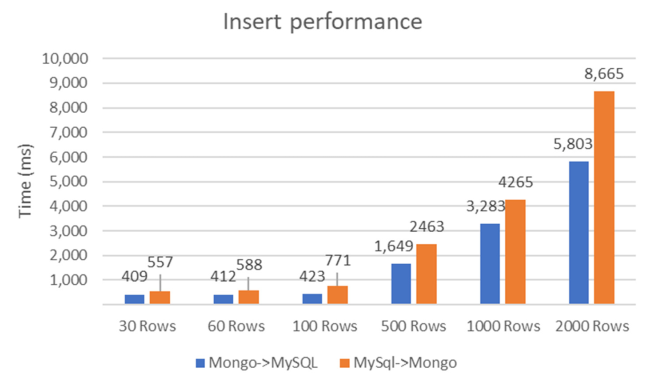
\includegraphics[width=0.85\textwidth]{gambar/bab1/chart-exponent}
  \caption{Grafik peningkatan operasi \emph{insert} pada \emph{database} berbeda, biasa disebut \emph{heterogenous} (\cite{Gyrdi2023})} 
\end{figure}

Waktu \emph{delay} antara sinkronisasi \emph{database} dapat diatasi dengan melakukan efisiensi terhadap 
algoritma sinkronisasi. Salah satu algoritma sinkronisasi yang dapat dicoba diterapkan adalah arsitektur dan algoritma sinkronisasi yang berada pada
\emph{paper Design and Implementation of a Heterogeneous Relational Database Synchronization Mechanism Based on Tree Distribution Architecture} (\cite{Xu2019}). 
Untuk menerapkan algoritma sinkronisasi tersebut juga akan membutuhkan lapisan sinkronisasi tambahan dikarenakan sqlite dan mongoDB merupakan entitas \emph{database}
yang berbeda. Lapisan tambahan ini bisa dihilangkan dengan memasukkan lapisan sinkronisasi tersebut sebagai fitur \emph{native} dari MongoDB dan SQLite.
Namun \emph{source code} MongoDB memiliki lisensi yang memiliki aturan-aturan tertentu ketika pengembang melakukan memodifikasi dan mengubah \emph{source code}.
Aturan-aturan pada lisensi membuat pengembang tidak bisa memiliki kendali penuh terhadap \emph{source code} sistem tersebut. Permasalahan ini yang memicu timbulnya ide untuk membuat \emph{database} baru yang dapat lebih 
adaptif terhadap sistem \emph{crawling} yang berjalan saat ini. Hal ini dikarenakan pengembang dapat memegang kendali penuh mulai dari proses pengambilan, penyimpanan,
pengubahan dan penghapusan data. Algoritma sinkronisasi antar \emph{database} pun juga dapat diterapkan langsung pada \emph{database} tanpa melalui perantara lapisan sinkronisasi.

Jika meninjau \emph{database} selain MongoDB yang memiliki lisensi lebih aman seperti Postgresql terdapat permasalahan baru yaitu kompleksitas dari \emph{source code}. Kompleksitas ini
berbanding lurus dengan banyaknya fitur postgresql, di dalam \emph{source code} tersebut terdapat banyak sekali \emph{file} serta \emph{function} yang dibuat. Oleh karena itu, untuk mencoba
mengadaptasi \emph{source code} dari postgresql dan mengubah sesuai dengan kebutuhan akan sulit dilakukan dengan kemampuan penulis saat ini. Selain itu, \emph{database engine} yang telah dibuat
biasanya telah memiliki alur lapisan pemrogamannya tersendiri. Sementara dengan membuat \emph{database engine} tersendiri, pengembang dapat menyesuaikan alur serta algoritma
yang sesuai dengan sistem \emph{crawling} pada penelitian sebelumnya (\cite{ridho2024})

% Paragraph 9
Lalu manfaat lain dari pembuatan \emph{database} baru ini adalah pengembang dapat menyesuaikan skema distribusi \emph{database} yang paling cocok dengan 
sistem \emph{crawling} yang ada saat ini (\cite{ridho2024}). Salah satu konsep distribusi \emph{database} yang dapat digunakan adalah konsep distribusi yang ada
pada \emph{paper} berjudul \emph{Research on The Improvement of MongoDB Auto-Sharding in Cloud Environment} (\cite{improvementsharding}). \emph{Paper}
ini membahas tentang arsitektur yang berjalan pada MongoDB. Konsep distribusi dilakukan dengan memecah 
kumpulan-kumpulan data menjadi potongan-potongan kecil. Potongan tersebut dapat didistribusikan antar mesin agar setiap mesin 
bertanggung jawab pada subset dari total data set yang ada. Penggunaan \emph{database} pada sistem terdistribusi akan diterapkan pada sistem \emph{crawling} ini berdasarkan 
saran dari penelitian sebelumnya (\cite{ridho2024}). Akan tetapi penerapan \emph{database} pada sistem terdistribusi baru akan dilaksanakan setelah mesin dan fitur utama dari 
\emph{database} baru ini selesai.

\section{Rumusan Masalah}
Berdasarkan dari rincian dan penjelasan latar belakang di atas, maka didapatkan 
rumusan masalah "\textbf{Bagaimana Perancangan dan Implementasi \emph{Prototype Database Engine} Berbasis 
\emph{Structure Oriented Programming} Menggunakan Rust?}".

\section{Batasan Masalah}
Rumusan masalah yang didapat memiliki permasalahan yang cukup banyak dan luas 
sehingga harus diperjelas batasaannya. Batasan Masalah pada penelitian yang 
dilakukan antara lain:
\begin{enumerate}
	\item{
		Pembuatan \emph{database engine} meliputi penerapan penyimpanan data 
		secara persisten dan menjaga integritas data yang dibuat dengan bahasa pemrograman 
		Rust.
	}
	\item{
		\emph{Database engine} yang dibuat belum menggunakan bahasa/\emph{query} secara langsung 
		sehingga jika ingin mengambil data hanya bisa melalui \emph(interface) yang 
		tersedia.
	}
	\item{
		\emph{Database} yang dibuat belum menerapkan \emph{foreign key} atau relasi antar tabel, 
		sehingga penerapan nanti tidak bisa memiliki \emph{constraint} antar tabel. Pengambilan 
		data antar tabel hanya sebatas \emph{joining} tabel.
	}
\end{enumerate}

\section{Tujuan Penelitian}
\begin{enumerate}
	\item{
		Membuat \emph{database engine} yang dapat digunakan secara \emph{universal} (Dapat digunakan pada sistem lain) dan memiliki data konsisten
	}
	\item{
		Membuat \emph{database engine} yang memiliki proses penyimpanan, pengambilan, pengubahan, penghapusan, \emph{joining} antar table dan memiliki \emph{indexing}.
	}
	\item{
		Membuat \emph{database engine} yang memiliki kendali penuh mulai dari tahap penyimpanan, pengambilan, pengubahan dan penghapusan. 
		Arti dari kendali penuh yang dimaksud adalah jika terdapat perubahan atau penambahan fitur ke depannya, maka tidak perlu melalui
		layer tambahan dan dapat ditambahkan ke pemrosesan \emph{database} secara langsung (\emph{seamless}).
	}
\end{enumerate}

\section{Manfaat Penelitian}
\begin{enumerate}
	\item Bagi penulis \\
	Menambah wawasan dan ilmu tentang sistem terdistribusi serta penerapannya, 
	memperoleh gelar sarjana pada bidang ilmu komputer dan mendapatkan pengalaman 
	dalam menulis sebuah jurnal ilmiah.
		
	\item Bagi Program Studi Ilmu Komputer \\
	Penelitian ini dapat menjadi referensi untuk penelitian yang akan dilakukan 
	mahasiswa ilmu komputer mendatang.


	\item Bagi Universitas Negeri Jakarta \\
	Dapat menjadi bahan evaluasi dan penilaian kualitas akademik di Universitas 
	Negeri Jakarta khusus nya pada program studi Ilmu Komputer.
			
\end{enumerate}

% Baris ini digunakan untuk membantu dalam melakukan sitasi
% Karena diapit dengan comment, maka baris ini akan diabaikan
% oleh compiler LaTeX.
\begin{comment}
\bibliography{daftar-pustaka}
\end{comment}
